\chapter{Szoftverfejlesztés}
A prototípus szoftverét kettéválasztottam a két működési mód szerint, az egyik a manuális vezérlést valósítja meg, a másik az automatikust. A kettő között lényeges különbségek vannak a prioritásokban. A kézi vezérlésnél a legfontosabb a valós idejű megjelenítés, és a minél gyorsabb reagálás a felhasználói parancsokra. Az automata működésnél a megjelenítés kevésbé fontos, viszont a képfelismerés és ez által a célpont követése kiemelkedő fontosságú.


\section{Használt Python modulok, eszközök}
\subsection*{OpenCV könyvtár \cite{opencv}}
Az \textbf{OpenCV} (Open Source Computer Vision Library) egy nyílt forráskódú könyvtár, amelyet eredetileg az Intel fejlesztett ki, és amelyet széles körben használnak a számítógépes látás (computer vision) és képfeldolgozás területén. Az OpenCV rendkívül sokoldalú eszközkészletet biztosít a képekkel és videókkal kapcsolatos különféle feladatok megoldásához, amelyet elsősorban C++-ban fejlesztettek ki, de támogat Python, Java, és MATLAB interfészeket is. A Python interfész különösen népszerű, mivel egyszerűsíti az OpenCV használatát gépi tanulási és mesterséges intelligencia-alkalmazásokban. A fő funkciói közé tartozik a képfeldolgozás, tárgy- és arcérzékelés, mozgáskövetés, valamint a 3D-s modellezés és képanalízis.\\

Az OpenCV architektúrája moduláris felépítésű, ami lehetővé teszi a különböző funkciók rugalmas használatát. A modulok között megtalálhatóak a képfeldolgozási, objektumfelismerési, gépi tanulási és 3D modellezési könyvtárak. A Pythonban a \code{cv2} könyvtárként importálható OpenCV API biztosítja a különböző funkciók egyszerű elérését, így akár néhány sor kóddal is gyors eredmény érhető el.\\

Többféle képformátumot támogat, például JPEG, PNG és BMP, és rendelkezik valós idejű video- és képadatok betöltésére szolgáló funkciókkal is, például a \code{VideoCapture} objektummal. Ez utóbbi lehetővé teszi, hogy közvetlenül kamerákból vagy videófájlokból dolgozzunk.\\

Az \textbf{OpenCV }használata igen elterjedt az iparban és a kutatásban is, többek között autonóm járművek, biztonsági rendszerek, gyártósori ellenőrző rendszerek, orvosi képalkotás és mobilalkalmazások terén. A könyvtár rugalmassága és széleskörű támogatása lehetővé teszi, hogy számos programozási és mérnöki területen is alkalmazható legyen, ahol képfeldolgozásra és gépi látásra van szükség.

\subsection*{Socket modul \cite{socket}}

Python \code{socket} modulja alacsony szintű hozzáférést biztosít a hálózati kommunikációhoz, lehetővé téve különböző típusú hálózati kapcsolatok létrehozását, beleértve az általam használt TCP-t és az UDP-t.\\

A \textbf{TCP} kapcsolat-orientált protokoll, amely biztosítja az adatok érkezési sorrendjét és helyességét. A \code{socket.SOCK\textunderscore STREAM} típust használjuk, ha TCP kapcsolatot szeretnénk létrehozni. A TCP kapcsolatok esetében a \code{connect()} függvény a kapcsolat kezdeti lépése, és a kliens-szerver kommunikáció folyamatosan fennmarad.\\

Az \textbf{UDP} kapcsolatnélküli protokoll, amely nem garantálja az adatok sorrendjét és integritását, viszont gyorsabb, mivel nincs szükség kapcsolatra. Az UDP kapcsolathoz a  \code{socket.SOCK\textunderscore DGRAM} típust használjuk, így a kliens és a szerver bármikor küldhet és fogadhat adatokat. Ideális valós idejű alkalmazásokhoz, ahol nem kritikus minden csomag megérkezése (pl. video streaming).\\

Mindkét típusnál a \code{send()}, \code{sendto()}, \code{recv()}, és \code{recvfrom()} függvények használhatók az adatok küldésére és fogadására.

\subsection*{Multiprocessing modul \cite{multiprocessing}}

A \textbf{multiprocessing} modul lehetővé teszi a Python számára, hogy párhuzamosan több folyamatot indítson el, ami segít a CPU-erőforrások jobb kihasználásában. A modul az operációs rendszer által kezelt különálló folyamatokat hoz létre, így azok külön memóriaterülettel rendelkeznek, és jobban teljesítenek többmagos processzorokon, mint a \textsl{threading} modul.\\ 

A \code{Process} osztály segítségével indíthatunk el új folyamatokat, amelyek egymástól függetlenül végrehajtanak egy adott funkciót. A modul támogatja az eseménykezelést, kommunikációs csatornákat (pl. \code{Queue}, \code{Pipe}) és szinkronizálást (pl. \code{Event}, \code{Lock}), amelyek segítségével a folyamatok egymással adatokat cserélhetnek és szinkronizálhatják működésüket.

\subsection*{Pygame modul \cite{pygame}}

A \textbf{pygame} egy multimédiás modul, amely elsősorban 2D játékok fejlesztésére alkalmas, de egyéb alkalmazásokkor is lehetőséget ad bemenetek kezeléséhez.\\

A \code{pygame.event.get()} függvény segítségével olvashatjuk le az egér- és billentyűzet-eseményeket, így például kattintások, gombnyomások és egérmozgások lekérdezése egyszerű. Az interaktív elemek kirajzolása és mozgatása egyszerű a \code{pygame.display.update()} és \code{pygame.draw} függvényekkel, amelyek lehetővé teszik grafikus objektumok megjelenítését a képernyőn. Magában foglalja a számítógépes grafikákat, a hang- és programkönyvtárakat, amiket a Python programozási nyelvre fejlesztettek ki. 

\subsection*{Pickle modul \cite{pickle}}
A \textbf{pickle} modul sorosítást és deszerializációt tesz lehetővé, azaz a Python-objektumok bináris formátumba alakítását és visszaalakítását.\\

A \code{pickle.dumps()} segítségével a Python-objektumokat bináris formátumba alakíthatjuk, amely lehetővé teszi azok egyszerű tárolását vagy átvitelét, például hálózaton keresztül. A \code{pickle.loads()} a bináris formátumú adatokat visszaalakítja eredeti Python-objektummá. A pickle használata előnyös lehet akkor, ha komplex adatszerkezeteket szeretnénk fájlban tárolni vagy hálózaton keresztül továbbítani.

\pagebreak

\section{Gépi látás}
A célpontfelismerés módszere volt az automata működés legfontosabb eleme. Elsősorban az OpenCV könyvtár különböző lehetőségeit vizsgáltam, ugyanis ez a legjobban kiforrott modul, amely könnyedén használható python programokban.

\subsection{Template matching \cite{templatematching}} \label{sec:soft_template}

A \textbf{Template Matching} (sablonillesztés) egy egyszerű, de hatékony módszer, amelyet statikus képekben keresett minták (sablonok) azonosítására használnak. Ez a módszer összehasonlít egy kisebb, előre meghatározott képrészletet (a sablont) a nagyobb képen található területekkel, és megkeresi a legjobban illeszkedő pozíciót.\\

\textbf{Működés:} Az OpenCV \code{cv2.matchTemplate()} függvényével kivitelezhető, amely végigfuttatja a sablont a célképen, és minden pixelpozíciónál egy hasonlósági pontszámot generál. A legmagasabb értékű pontszám mutatja az illeszkedés helyét.\\

\textbf{Előnyei:} Gyors és könnyen implementálható, különösen ismert méretű és orientációjú objektumok azonosításához.\\

\textbf{Korlátozások:} Gyengén teljesít forgatott, méretarányosan eltérő vagy eltorzult objektumoknál, valamint változó fényviszonyok mellett.

\subsection{Feature Matching \cite{featurematching}} \label{sec:soft_feature}

A \textsl{Feature Matching} (jellemzőpont-illesztés) egy kifinomultabb módszer a képjellemzők összehasonlítására és egyeztetésére. A módszer a két képben található pontokat (feature-ket) párosítja, ezáltal lehetővé teszi forgatásokkal, elforgatásokkal és méretarányokkal szembeni robusztus egyeztetést.

\textbf{Működés:} Először meghatározzuk a képen lévő fontos jellemzőpontokat (például élek, sarkok), amelyeket különböző detektorok (például SIFT, SURF vagy ORB) segítségével találhatunk meg. Ezután az \code{cv2.BFMatcher()} (Brute Force Matcher) vagy a \code{cv2.FlannBasedMatcher()} függvénnyel azonosítjuk a jellemzőpontokat.\\

\textbf{Előnyei:} Robusztus a forgatásokkal, skálázással és elmozdulásokkal szemben, így alkalmas tárgyak nyomon követésére és objektumok felismerésére különböző nézetekből.\\

\textbf{Korlátozások:} A nagy számítási igényű algoritmusok miatt lassabb lehet, különösen nagy méretű képeken.

\subsection{Target Tracking \cite{targettracking}} \label{sec:soft_target}

A \textsl{Target Tracking} (célkövetés) feladata egy mozgó objektum követése egy videófolyamon vagy valós idejű képforráson keresztül. Az OpenCV több nyomon követési algoritmust is biztosít, amelyek segítenek abban, hogy a kiválasztott objektumot stabilan követni tudjuk, még akkor is, ha változik a pozíciója vagy a környezeti fény.

Algoritmusok:
\begin{list}{-}{}
	\item Mean Shift: A \code{cv2.meanShift()} függvénnyel elérhető algoritmus egy adott objektum körüli eloszlás csúcsértékeit keresi, és folyamatosan frissíti a helyét.
	\item CamShift (Continuously Adaptive Mean Shift): \code{A cv2.CamShift()} algoritmus a Mean Shift továbbfejlesztett változata, amely figyelembe veszi az objektum méretének és alakjának változásait.
	\item Modern nyomkövetési algoritmusok: Az OpenCV 3.x-es és újabb verziói lehetővé teszik algoritmusok használatát, mint a KLT (Kanade-Lucas-Tomasi) nyomkövető, a CSRT és a MedianFlow, amelyek kifejezetten valós idejű és pontos követést biztosítanak.
\end{list}

\textbf{Előnyei:} Alkalmas valós idejű alkalmazásokhoz, mint például a videó megfigyelés vagy az autonóm rendszerek, ahol a cél folyamatosan mozgásban van.

\textbf{Korlátozások:} Bizonyos algoritmusok hajlamosak elveszteni a célpontot gyors mozgásoknál vagy hirtelen pozícióváltásoknál.
\subsection{Haar cascade \cite{haarcascade}} \label{sec:soft_haar}

A \textsl{Haar Cascade} módszer az egyik legelterjedtebb technika az objektumfelismerésre, különösen az arcfelismerésben. A gépi tanuláson alapuló módszer képes egy képben vagy videófolyamon objektumokat megtalálni azáltal, hogy mintákat ismer fel az előképzett adatok alapján.\\

\textbf{Működés:} A Haar-cascade egy többlépcsős osztályozó, amelyet sok pozitív és negatív mintából tanítanak be. \code{A cv2.CascadeClassifier()} osztály segítségével előre tanított modelleket, például arcokat, szemeket vagy különböző objektumokat kereshetünk.\\

\textbf{Gépi tanulás:} A módszer előnye, hogy nagyon hatékonyan képes felismerni az objektumokat. A gépi tanulás során a kimeneti modell jellemzőit úgy optimalizálják, hogy gyorsan tudja felismerni a keresett objektumokat még zajos vagy eltérő körülmények között is.\\

\textbf{Előnyei:} A Haar-cascade módszer jól használható olyan alkalmazásokhoz, ahol előre meghatározott objektumokat (például arcokat) kell azonosítani. Nagy előnye, hogy valós időben is képes futni.\\

\textbf{Korlátozások:} Hajlamos a pontatlan felismerésre, ha az objektumok perspektívája, megvilágítása vagy pozíciója jelentősen eltér az előképzett mintáktól. Alternatív megoldásként mélytanulási módszerek (például konvolúciós neurális hálózatok) használhatók az ilyen problémák javítására. \pagebreak



\section{A szoftver működése}
A rendszer két alapvető részből áll: egy számítógépből (PC), amely felhasználói interfészként szolgál az operátor számára, és egy Raspberry Pi-ből, amely a fegyverrendszer vezérlését és képátvitelét végzi. A két eszközön futó program között két folyamat kommunikál, két különböző porton: egy UDP protokoll alapú adatátvitel a videó küldéséhez, illetve egy TCP alapú a vezérlőparancsok fogadásához. \\

\subsection{A PC-n futó program működése}
A PC-s kód \code{main()} függvénye két külön folyamatot indít: egy videó-fogadó folyamatot és egy vezérlő-küldő folyamatot, melyek egy multiprocessing-eseményjelző (\code{stop\textunderscore event}) segítségével állnak meg szükség esetén. A két folyamat használ közös erőforrást, a \code{frame\textunderscore queue}-t, amelybe a videó-fogadó betölti a Raspberry-ből kapott képkockákat, a Pygame pedig felhasználja az a másik folyamatban. A felső szint folyamatábrája a \ref{fig:PC_main}. ábrán látható. 

\begin{figure}[h!]
	\centering
	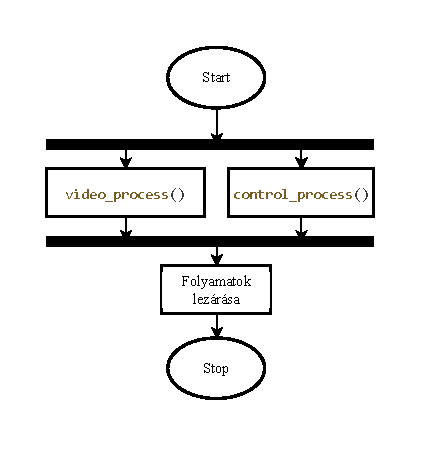
\includegraphics{PC_main}
	\caption{A PC-n futó program felső szintű folyamatábrája}
	\label{fig:PC_main}
\end{figure}

\subsubsection*{Videó-fogadó folyamat}

A videó-fogadó folyamat (\code{video\textunderscore receiver}) UDP-n keresztül kapja a képkockákat, amelyek a Raspberry Pi-ről érkeznek csomagokra bontva. A folyamat összegyűjti ezeket a csomagokat, majd a kép adatokat újraegyesíti és és betölti a \code{frame\textunderscore queue}-ba. Az UDP protokoll nagy sebességet tud elérni, de nem garantált a célba érés. A videó esetében azonban ez nem probléma, ha elveszik egy képkocka attól még értelmezhető marad a videó. A folyamat a következőképpen működik:

\begin{list}{$\bullet$}{}
	\item A folyamat egy UDP socketet (\code{video\textunderscore socket}) hoz létre a megadott porton.
	\item Egy ciklusban fogadja a képkockák csomagjait, minden egyes csomag egy fejlécet és a kép adatrészleteit tartalmazza.
	\item A fejléc alapján a folyamat azonosítja a csomagokhoz tartozó képkockát és azok sorrendjét. A bufferben gyűjtött csomagokat az összes részlet megérkezése után egyesíti.
	\item Az egyesített képkockát visszafejti (unpickling és JPEG dekódolás), majd a képre helyez egy célkeresztet a \code{cv2.line()} függvény alkalmazásával.
	\item A teljes képkockát behelyezi a \code{frame\textunderscore queue} sorba, a \code{.put()} metódussal.
\end{list}

A folyamatábra a \ref{fig:PC_videoreceiver}. ábrán látható.

\begin{figure}[h!]
	\centering
	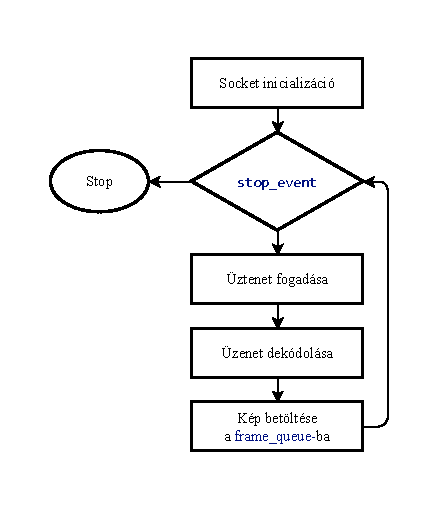
\includegraphics{PC_videoreceiver}
	\caption{A \code{video\textunderscore receiver} függvény folyamatábrája}
	\label{fig:PC_videoreceiver}
\end{figure}

\subsubsection*{Vezérlés-küldő folyamat}

A vezérlés-küldő folyamat (\code{control\textunderscore sender}) a felhasználó irányítási parancsait továbbítja a Raspberry Pi felé. A folyamat a Pygame könyvtár segítségével észleli az egér- és billentyűeseményeket, majd a megfelelő parancsokat TCP csomag formájában küldi a Raspberry Pi irányába. Ezentúl felelős a HUD megjelenítéséért, amiről a felhasználó le tudja olvasni a prototípus állapotát. A folyamat illusztrációja a \ref{fig:PC_controlsender}. ábrán látható.\\


\begin{figure}[h!]
	\centering
	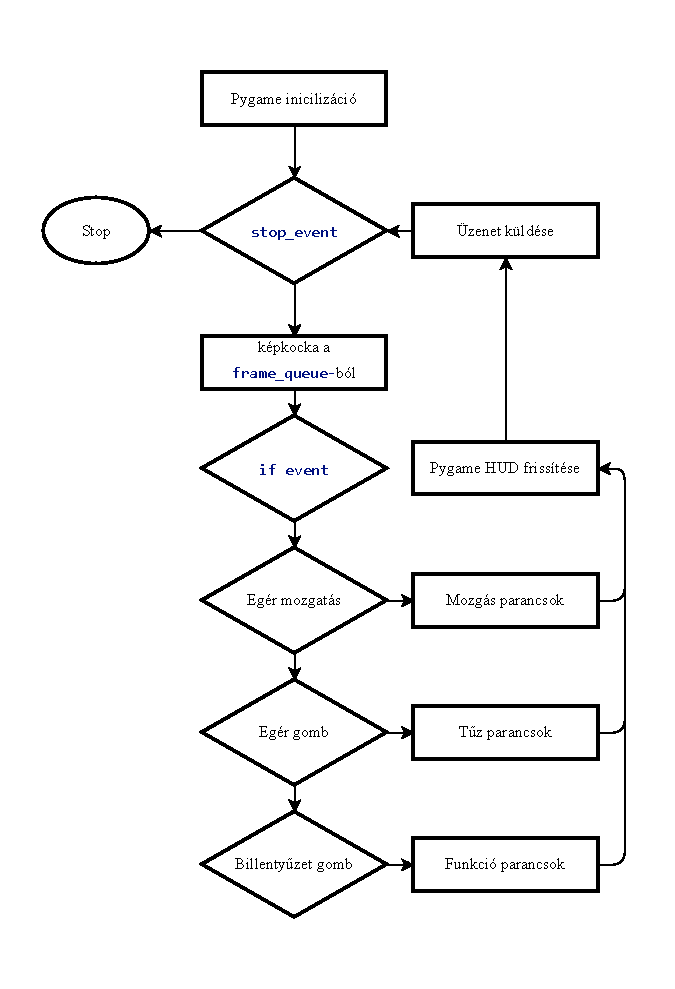
\includegraphics{PC_controlsender}
	\caption{A \code{control\textunderscore sender} függvény folyamatábrája}
	\label{fig:PC_controlsender}
\end{figure}

A felhasználó számára fontos, hogy minden információt le tudjon egyből olvasni a fegyver működéséről, így ezeket a PyGame ablakon megjelenítettem (\ref{fig:teszt_manual1}. ábra). Itt látható:

\begin{figure}[h!]
	\centering
	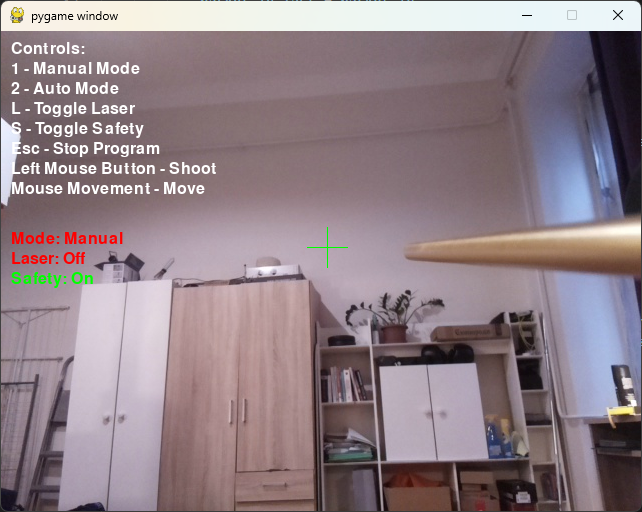
\includegraphics[width=0.5\linewidth]{teszt_manual2}
	\caption{Pygame HUD}
	\label{fig:teszt_manual1}
\end{figure}


\begin{list}{-}{}
	\item Használható parancsok és a hozzájuk rendelt gombok
	\item Milyen módban működik a rendszer
	\item Biztosítva van-e a rendszer
	\item Működik-e a lézer
\end{list}

A PyGame ablak háttere pedig az éppen utolsó képkocka, amit a videó-fogadó folyamat a \code{frame\textunderscore queue}-ba tett. A vizuális megjelenítés mellett a folyamat feladata a parancsok küldése, ezek a következőek lehetnek:

\begin{list}{-}{}
	\item Az egér mozgása esetén \code{MOVE} parancs az X és Y elmozdulási adatokkal, így irányítva a fegyver mechanikai elmozdulását.
	\item Az bal egérgomb lenyomásakor (\code{SHOOT\textunderscore START}, a felengedésekor \code{SHOOT\textunderscore STOP}) parancsot adhatunk ki, értelemszerűen a tüzelés megkezdésére és befejezésére.
	\item A billentyűzet gombjaival a lézert, (\code{LASERTOGGLE}) a biztosítást (\code{SAFETY}), illetve a működési módokat lehet állítani(\code{MANUALMODE} és \code{AUTOMODE}).
	\item Amikor a felhasználó az ESCAPE gombot megnyomja, a folyamat küld egy leállítási parancsot (\code{STOP}), majd befejezi működését.
\end{list}

A program a működési módtól függetlenül működik, mindig ugyanazokat az üzeneteket küldi el. A kliens programtól függ, hogyan értelmezi azokat.

\pagebreak

\subsection{A Raspberry Pi-n futó program működése}
A Raspberry Pi-n több folyamat is fut: Egy videó-küldő, egy vezérlés-fogadó, egy célpontfelismerő, illetve egy motormozgató. A közös erőforrások között szintén van egy \code{stop\textunderscore event} eseményjelző, amely minden folyamat megállításáért felelős. Ezentúl van a \code{frame\textunderscore queue} és a \code{pos\textunderscore queue}, amelyek tartalmazzák a képkockákat és a felismert célpont pozícióját. A \code{main()} függvény illusztrációja látható a \ref{fig:RPI_main}. ábrán.

\begin{figure}[h!]
	\centering
	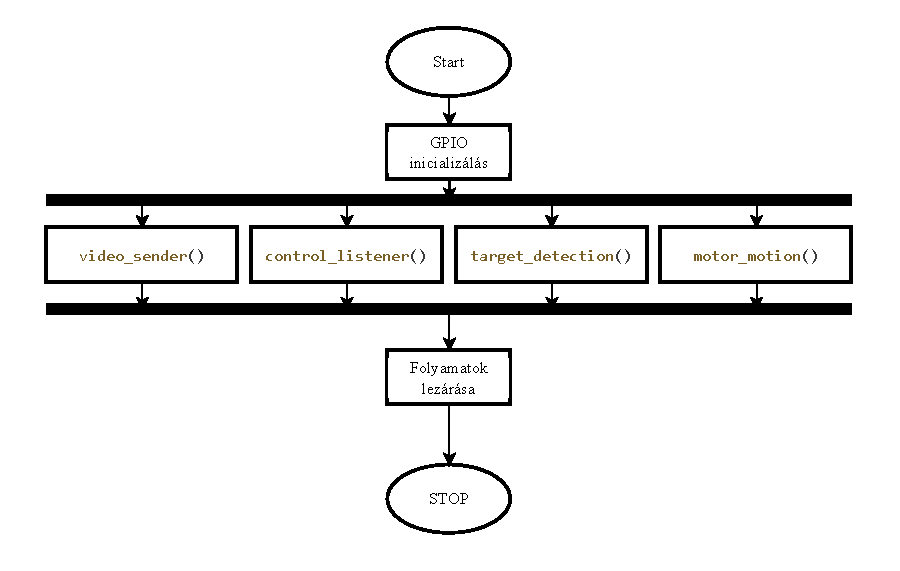
\includegraphics{RPI_main}
	\caption{A Raspberry PI-n futó program felső szintű folyamatábrája}
	\label{fig:RPI_main}
\end{figure}

\subsubsection*{Célfelismerő folyamat}

A \code{target\textunderscore detection()} folyamat felelős az arcok felismeréséért, és a helyzetük meghatározásához.

\begin{list}{-}{}
	\item A \code{cv2.CascadeClassifier()} függvénnyel betölti az előre betanított \textsl{haarcascade\textunderscore frontalface\textunderscore default.xml} modellt
	\item A \code{frame\textunderscore queue.get()} metódussal kiveszi az utolsó képkockát a sorból
	\item A \code{cv2.detectMultiScale()} megtalálja az arcokat a képkockán
	\item Méret szerint sorba rendezi az arcokat, és kiszámolja a legnagyobb pozícióját
	\item Betölti a pozíciót a sorba a \code{pos\textunderscore queue.put} metódussal
\end{list}

Ez a folyamat csak akkor fut, hogyha az \code{automode\textunderscore event()} flag be van állítva, tehát az eszköz automatikusan működik. A folyamat illusztrációja a \ref{fig:RPI_targetdetection}. ábrán látható

\begin{figure}[h!]
	\centering
	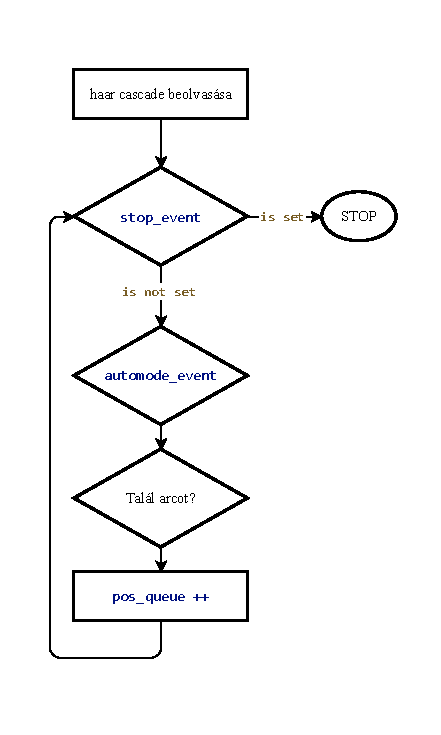
\includegraphics{RPI_targetdetection}
	\caption{A \code{target\textunderscore detection} függvény folyamatábrája}
	\label{fig:RPI_targetdetection}
\end{figure}


\subsubsection*{Vezérlés-fogadó folyamat}

A \code{control\textunderscore listener} folyamat először , a rendszer indításakor elvégzi a fegyver pozíciójának beállítását. A motorokat addig forgatja, amíg a végálláskapcsolók nem adnak jelet. Ezután pedig, miután tudjuk a pontos pozíció, visszaforgatja a fegyvert középre, és nullázza a \code{POSX} és \code{POSY} globális változókat. Ezután pedig TCP-n keresztül fogadja a PC-ről érkező irányítási parancsokat, és a megfelelő fizikai komponenseket működteti, majd a rendszer leállításakor újra középre állítja a fegyvert. A következő parancsokat tudja fogadni, attól függően, hogy melyik módban működik a prototípus. 

\begin{list}{-}{}
	\item A parancs típusa alapján (\code{MOVE}, \code{SHOOT\textunderscore START}, \code{SHOOT\textunderscore STOP},  \code{LASERTOGGLE}, \code{ STOP}) különböző műveleteket hajt végre.
	\item \code{MOVE} parancs esetén az X és Y elmozdulási értékek alapján irányítja a két DRV8825 motorvezérlő áramkört, így mozgatva a fegyvert az elvárt irányba.
	\item A lövésvezérlés (\code{SHOOT\textunderscore START} és \code{SHOOT\textunderscore STOP}) esetén aktiválja vagy deaktiválja a fegyver LED-jét.
	\item A lézerkapcsolás (\code{LASERTOGGLE}) a lézerdiódát ki- vagy bekapcsolja.
	\item Amennyiben \code{STOP} parancs érkezik, a folyamat leállítja a működését.
\end{list}

A függvény folyamatábrája a \ref{fig:RPI_controllistener}. ábrán látható.

\begin{figure}[h!]
	\centering
	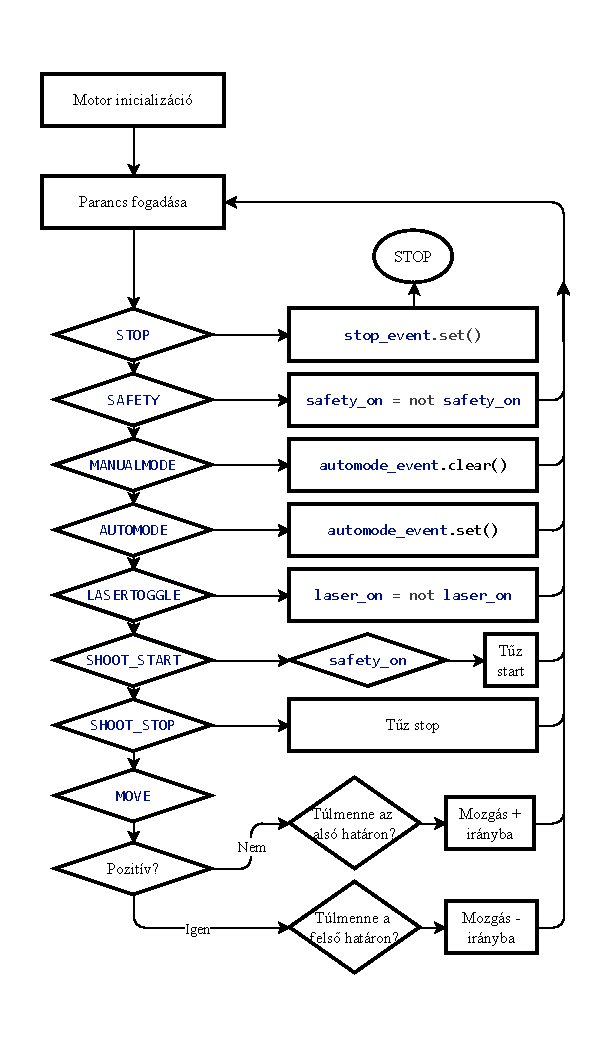
\includegraphics{RPI_controllistener}
	\caption{A \code{control\textunderscore listener} függvény folyamatábrája}
	\label{fig:RPI_controllistener}
\end{figure}


\begin{list}{-}{}
	\item \code{STOP} parancs esetén az \code{stop\textunderscore event}-et beállítja, ezzel leállítva az összes folyamatot
	\item \code{AUTOMODE} parancs esetén az \code{automode\textunderscore event}-et igazra állítja
	\item \code{MANUALMODE} parancs esetén az \code{automode\textunderscore event}-et hamisra állítja
	\item \code{MOVE} parancs esetén az X és Y elmozdulási értékek alapján irányítja a két motorvezérlőt, így mozgatva a fegyvert a megfelelő irányba.
	\item A (\code{SHOOT\textunderscore START} és \code{SHOOT\textunderscore STOP}) esetén aktiválja vagy deaktiválja a fegyvert. Aktiválni csak akkor lehet, ha a \code{safety\textunderscore on} hamis.
	\item A (\code{LASERTOGGLE}) a lézerdiódát ki- vagy bekapcsolja.
	\item Amennyiben \code{SAFETY} parancs érkezik, beállítja a \code{safety\textunderscore on} flag-et.
\end{list}

A végtelen ciklus ellenőrzi a \code{stop\textunderscore event} flag-et, és ha igaz lesz, akkor kilép belőle. Ekkor a \code{TurnStep()} fügvénnyel addig lép, amíg középen nem lesz a fegyver, valamint a lézert is lekapcsolja.

\begin{figure}[h!]
	\centering
	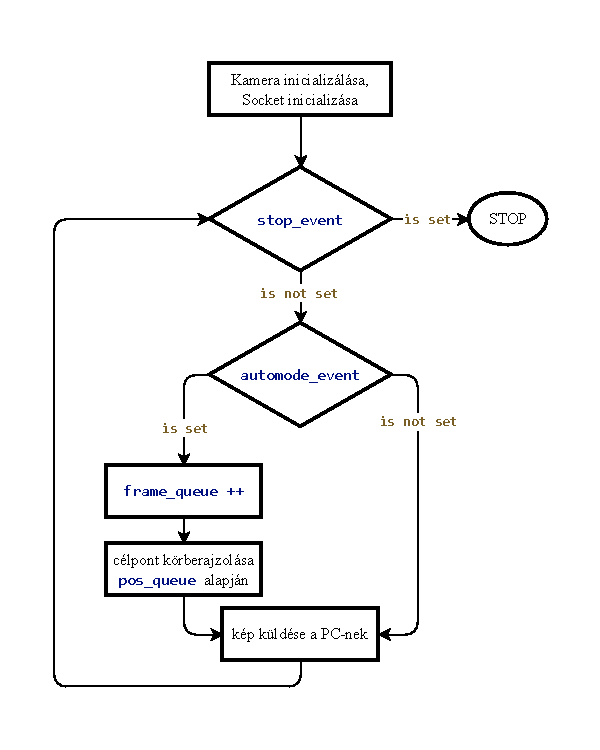
\includegraphics{RPI_videosender}
	\caption{A \code{video\textunderscore sender} függvény folyamatábrája}
	\label{fig:RPI_videosender}
\end{figure}

\subsubsection*{Videó-küldő folyamat}
A videó-küldő folyamat (\code{video\textunderscore sender}) a Raspberry Pi kamerájából érkező képet szerzi meg és osztja meg a PC-vel UDP kapcsolaton keresztül. A folyamat illusztrációja a \ref{fig:RPI_videosender}. ábrán látható.

\begin{list}{-}{}
	\item A kamerakép feldolgozása során a kód rögzíti az egyes képkockákat, amelyeket JPEG formátumba kódol és pickle segítségével tömörít.
	\item Amennyiben az \code{automode\textunderscore event} flag igaz, akkor beteszi a legutolsó képkockát a \code{frame\textunderscore queue}-ba, és a \code{pos\textunderscore queue} legutolsó elemei alapján húz egy téglalapot illeszt a képkockára, ezzel jelezve a talált arcot.
	\item Az adatok nagy mennyiségét figyelembe véve a képkockákat kisebb csomagokra bontja, amelyekhez megfelelő fejlécek tartoznak.
	\item A fejlécekben megtalálható a csomag azonosítója, amely segít a PC-n futó videó-fogadó folyamatnak a csomagok megfelelő sorrendbe állításában és összerakásában.
	\item A csomagokat a megadott IP-címre és portra küldi, és minden új képkockához új azonosítót rendel.
\end{list}

\begin{figure}[h!]
	\centering
	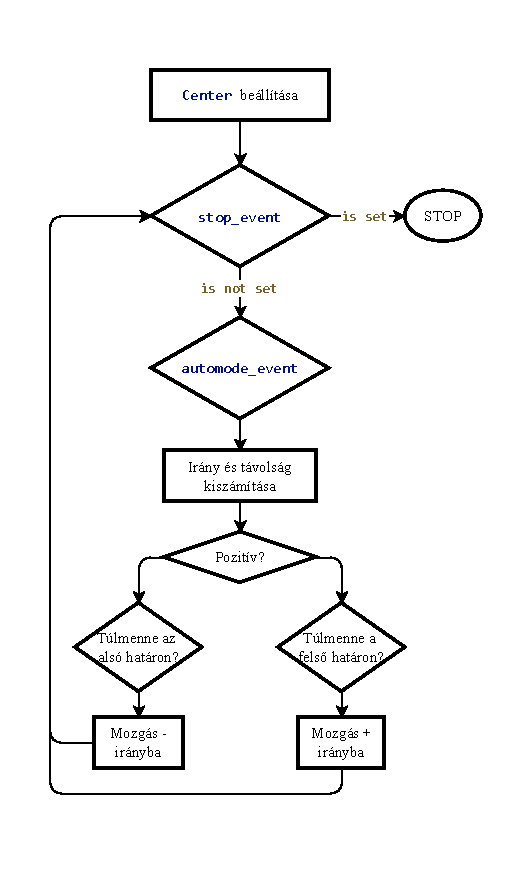
\includegraphics{RPI_motormover}
	\caption{A \code{motor\textunderscore motion} függvény folyamatábrája}
	\label{fig:RPI_motormover}
\end{figure}


\subsubsection*{Motormozgató folyamat}
A \code{motor\textunderscore motion()} folyamat azért felelős, hogy automata működés során mozgassa a motorokat, a kamera képe alapján. Azért gondoltam, hogy jobb így külön kezelni, mert az automata és kézi vezérlés mozgásának nagyon különböző a logikája. A folyamat működése a következőképpen működik:

\begin{list}{-}{}
	\item Kiolvassa a legutolsó pozíciót a \code{pos\textunderscore queue}-ből, majd a pozícióból és a középpont különbségéből kiszámítja a távolságot.
	\item Amennyiben a fegyver pozíciója a mozgásterületen belül van, a megfelelő irányba mozdul a távolsággal arányosan.
\end{list}

A motor csak akkor mozog, ha egy bizonyos értéknél nagyobb a távolság, így kerültem el, hogy folyamatosan rángatózzon az eszköz. Ez a folyamat is csak akkor fut, hogyha a \code{automode\textunderscore event} igaz. A folyamat illusztrációja a \ref{fig:RPI_motormover}. ábrán látható.

